
\chapter{Identification From in-Patient Reference Data}
\label{sec:PilotExperimentalIdentification}


Feasibility of uncertainty identification from virtual data has already been established, but validation on clinical data is required for the implementation of model-based controllers, which depend on the accuracy of the individual model obtained for each patient. However, model individualization has been proven difficult for data-based models \cite{stahl2009diabetes,percival2010modeling,finan2009experimental} or physiology-based models \cite{palerm2006robust}. Furthermore, suitability of classical metrics such as Mean Square Error for model evaluation has recently been questioned in the context of diabetes \cite{del2012glucose} where clinical implications of prediction errors must be considered.

Genetic algorithms for multiobjective optimization have been proven useful, but the computation times of this sort of optimizations are very long. In the virtual identification paradigm described in Chapter \ref{sec:InSilicoIdentification}, where only one optimization was needed for each patient, the use of multiobjective optimization was affordable and given that these techniques provide much more information of the optimization indexes that a single objective optimization, its use was encouraged. In this chapter however, several optimizations are needed for each patient in order to complete a full cross-validation study. From a practical point of view, there is no need to compute all individual possibilities in the Pareto Front to complete the cross-validation study. Therefore, the use of a composite index optimization is explored in this chapter, based on the paradigm described in the previous chapter

%There are two main barriers to individual patient's model identification: error/noise sources in the measurement devices (especially with the use of CGM devices for ambulatory data acquisition), and uncertainty/variability in the patient's behavior because of circadian rhythms and other non-modeled dynamics, such as alterations in the endocrine system, changes in daily life, stress, illness, etc. In this chapter, the feasibility of interval model identification for the characterization of intra-patient variability is investigated in clinical data. The minimization of a composite cost index comprising: (1) the glucose envelope width predicted by the interval model, and (2) a Hausdorff-distance-based prediction error with respect to the envelope, is proposed. A cross-validation study is performed for the evaluation of the method using clinical data from 12 patients with type 1 diabetes who underwent four in-clinic mixed meal tests with standardized initial conditions. CGM uncertainty is ignored as this work is considered to be a pilot identification study, hence the complexity of the experiment is reduced to a minimum. CGM influence on the identification from clinical data is reviewed later on this thesis.


\section{Optimization and index definition}
\label{sec:OptimizationAndIndexDefinition}
	
The dataset used for identification has been quickly introduced before in this thesis, and further details can be found in \cite{paoloibolus2012}. This data consisted in four monitored postprandial periods for twelve subjects with type 1 diabetes under CSII. On two occasions the patients received a mixed meal containing 40 g of CHO. On the other two occasions they ate a meal with the same relative macro-nutrients composition but with greater CHO content (100 g). For each meal, either a standard bolus or a computer-generated bolus-basal combination was administered following randomization. Pre-prandial plasma glucose was set around 100 mg/dL by means of a manual feedback intravenous insulin infusion. Hypoglycemia was avoided by using intravenous glucose infusion in case the patient's glucose levels were decreasing rapidly towards hypoglycemic levels. Plasma glucose was measured for 5 hours after the meal, every 5 minutes the first two hours after the meal and every 10 minutes afterwards, using a reference method (YSI 2300 STAT Plus Glucose analyzer, Yellow Springs Instruments, Ohio, USA). Plasma insulin was also measured periodically (every 15 minutes the first two hours, and every 30 minutes afterwards) along all the duration of the experiment. 

Due to the different sampling periods of the measurements, cubic spline interpolation was applied in order to get sample-per-minute data on all variables. Due to the high accuracy of YSI measurements \cite{nowotny2012precision} uncertainty modeling effort can be focused only in model inaccuracies and within-patient variability, disregarding uncertainty in the initial measurements.

As in the previous chapter, the interval version of the Cambridge model \cite{calm2010comparison,de2012prediction} was used. They provide a tight guaranteed envelope $[\underline{G} ,\overline{G}]$ for uncertain model inputs and model parameters $\mathbb{P}$. Plasma insulin was available for all the experiments in the dataset, so the insulin absorption model was not used in this identification for sake of simplicity. This reduces the identification and simulation of results to only 2 sub-models: the Cambridge endogenous model and the Cambridge glucose absorption model.

	
% Identification of interval models has been traditionally addressed under the framework of bounded-error identification [17], i.e., the set of parameter values consistent with a given %acceptable bound on the prediction error is computed:
%
%\begin{equation}
%\mathbb{P}=\left\{ \mathbf{p} \in \mathbb{R}^{n_p} \left| y(t_i ;\mathbf{p}) - y^{\ast}(t_i) \right| \leq e_i \right\}
%\label{eq:parameterset}
%\end{equation}
%	
%where $p$ is the parameter vector of dimension $n_p$, $y^{\ast}(t_i)$ and $y(t_i ;\mathbf{p})$ are the measurement and model prediction, respectively, at sample $i$ and $e_i$ is the %acceptable prediction error bound. However, when large intra-patient variability is present no consistent parameter values will generally be found. If for the same meal and insulin dose %the patient behaves very differently, no intersection between the acceptable output intervals will exist yielding an empty set for $\mathbb{P}$.

Following the notation introduced in the previous chapter, the cost index to be minimized is thus defined as:
\begin{equation}
	J_{we} (\mathbb{P}):=J_w (\mathbb{P})+\gamma \cdot J_e (\mathbb{P})		
\label{eq:JWE}
\end{equation}
where $\gamma$ is a weighting factor between the minimization of the envelope width ($J_w (\mathbb{P})$) and the fitting error ($J_e (\mathbb{P})$), resulting in the compound index ($J_we (\mathbb{P})$). A very small value for $\gamma$ yields to very small intervals for the identified model parameters $\mathbb{P}$ with loose data fitting, while large values of $\gamma$ provide good coverage of the data with large intervals for $\mathbb{P}$. The weight $\gamma$ has to be tuned a priori and it will define the degree of relaxation given to the optimization problem. In this chapter, a battery of in-patient identifications was run using several different weighting factors $\gamma$. Then, the authors decided to set $\gamma$=100 considering that the fitting results displayed a good compromise between the envelope width and data compliance.

Minimization of the cost index was performed with the global optimization algorithm Evolution Strategy with Covariance Matrix Adaptation (CMAES) (chapter \ref{sec:CovarianceMatrixAdaptativeEstimation}). The optimization to be performed is a non-linear single objective minimization with linear restrictions in the parameters (intervals). CMAES performs very fast optimizations on a single objective, with quadratic increment in the computation time with the number of parameters. Unfortunately, the build released by Hansen \textit{et al.} \cite{hansen2004evaluating} does not implicitly consider restrictions neither in the outputs nor in the inputs, so they have to be integrated in the cost index. Interval parameters consist of two independent parameters, upper and lower bounds, where obviously all the lower bounds must be smaller than their respective upper bounds. These greater-or-equal restrictions were checked first in the evaluation of the optimization index. If any of the lower bounds were superior to its upper bound, the index was declared invalid (set to NaN), and penalized greatly in the search \cite{hansen2004evaluating}. The final cost index is shown next:
\begin{equation}
J(\mathbb{P}):= \begin{cases}
\text{NaN} & \text{if} \; \overline{p_i} < \underline{p_i} \\
J_{we}(\mathbb{P}) & \text{otherwise}\\
\end{cases}
\label{eq:totalindex}
\end{equation}	
where $\overline{p_i}$ and $\underline{p_i}$ represent the upper and lower bounds of the parameter $p_i$. 

Meal absorption is a highly complex physiological process as demonstrated by dual and triple tracer studies. However, to date, only relatively simple models fitted for specific meals are available. Besides, estimation of carbohydrates intake by the patient is a big source of uncertainty. It is thus expected a great extent of uncertainty in model parameters $Bio$, $t_{maxG}$ and model input $D_g$.

As the experimental data were taken under controlled conditions, it can be justified here to consider no misestimation of the grams of CHO ingested (real-valued $D_g$) eliminating a big confounder of uncertainty.

Besides, two different time constants $t_{maxG40}$ and $t_{maxG100}$ were considered for the meals of 40 and 100 grams of carbohydrates, respectively, to account for possible non-linearity with respect to meal size. However, since only one meal of 40 g or 100 g would remain for identification considering that one day is left for validation purposes, variability in $t_{maxG40}$ and $t_{maxG100}$ cannot be expressed adequately by the available data, thus making their identification as intervals questionable. For this reason they were also considered real-valued. 
Uncertainty in the gastrointestinal system was then considered as an interval scale factor $\alpha$ multiplying the glucose absorption rate $G_{ex}(t)$. This means that an envelope is produced from the rate of appearance resulting from an identified gastrointestinal model with real-valued parameters. Pilot simulations suggest that this aggregation of uncertainty into a single parameter $\alpha$ may be considered equivalent to parametric uncertainty in $Bio$ and $t_{maxG}$ and similar data fitting capabilities are expected. Indeed, looking at Figure \ref{fig:tmaxvsalpha}, little difference between the simulation bands of either parameter is observed. Furthermore, this allows a significant reduction in the number of interval parameters in the identification problem, and thus in the computational cost.

\begin{figure}[hbtp]
\centering
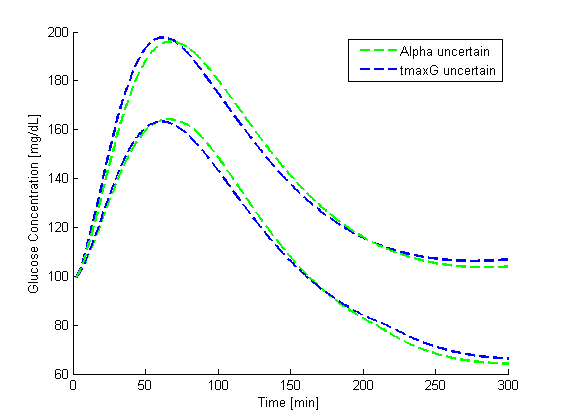
\epsfig{file=Figures/tmaxvsalpha.png, width=0.8\textwidth}\caption{Simulation of a postprandial period considering a 15\% uncertainty either in the parameter $t_{maxG}$ (in blue) or in the aggregated parameter $\alpha$ (green). Parameter $Bio$ is directly proportional to the aggregated parameter $\alpha$, so the uncertainty in the simulation is equivalent for both parameters.}
\label{fig:tmaxvsalpha}
\end{figure}

Description of uncertainty in the insulin and endogenous subsystems was considered in the insulin sensitivity parameters $S_{IT}$, $S_{ID}$ and $S_{IE}$, and the glucose transport among compartments $k_{12}$.

Identification of physiological models in diabetes often suffers from identifiability issues, especially when no tracer data is available and meal intake and insulin delivery is concomitant, as in this case. In order to test the ability of the method to properly characterize the source of uncertainty from only insulin and glucose data, two different scenarios were considered:

\begin{enumerate}
	\item In Scenario 1 implicit uncertainty in the gastrointestinal (interval value for $\alpha$), insulin and endogenous subsystems was considered.
	\item In Scenario 2 only uncertainty in the insulin and endogenous subsystems was considered ($\alpha$=1).
\end{enumerate}

This is illustrated in Table \ref{tab:listparameters}. Parameters marked as ``Interval''  were identified as uncertain (interval values), while parameters marked as ``Real'' were identified as real-valued parameters. Parameters not listed or, listed as ``Fixed'' were not identified and maintained in their nominal values throughout the identification and validation process.

\begin{table}[hbtp]
	\centering
	\begin{tabular}{| c | c | c |}
	\hline
	\textbf{Parameters} & \textbf{Scenario 1} & \textbf{Scenario 2} \\
	\hline
	$S_{IT}$ & Interval & Interval \\
  $S_{ID}$ & Interval & Interval \\
	$S_{IE}$ & Interval & Interval \\
	$k_{12}$ & Interval & Interval \\
	$\alpha$ & Interval & Fixed \\
	$t_{maxG40}$ & Real & Real \\
	$t_{maxG100}$ & Real & Real \\	
	$V_g$ & Real & Real \\		
	\hline 
	\end{tabular}
\caption{List of parameters to be identified in each scenario. ``Interval'' stands for parameters identified with uncertainty. ``Real'' are traditional parameters identified. ``Fixed'' stands for parameters not being identified.}
\label{tab:listparameters}
\end{table}
	
Out of the 4 days of monitoring available, only 3 were used for identification, while one day was kept apart for validation purposes (``leave-one-day-out'' cross-validation). A few pilot optimizations showed that identifications were much more accurate when the first 30 minutes of each postprandial period were excluded for fitting the data, which may be due to non-modeled dynamics.

All possible permutations for the identification-validation days were used, obtaining a \textbf{full cross-validation} study for all the patients and all the postprandial periods. Henceforth, the different permutations are denoted by the validation day number. Thus, permutation 3 uses days 1, 2 and 4 for identification, and validates with day 3. All the permutations of identification-validation days were performed twice for testing the repeatability of the results.

Six different measures were computed from the identification and validation days in order to evaluate the fit quality and model prediction ability, respectively:

\begin{enumerate}
	\item Width [mg/dL]:  maximum width of the glucose envelope generated by the identified interval model. It represents the patient's uncertainty for the postprandial period 
	\item Predictions [\%]: number of glucose measurements included inside the predicted glucose envelope.
	\item MARDout [\%]: relative error of the samples that were not well predicted and fell out of the glucose envelope. It complements the Predictions measure. For example, if Predictions is low but MARDout is also low, the data may follow the dynamics of the model, but with an offset that forces the data out of the prediction band. 
	\item MARDtot [\%]:  relative error for all the glucose measurements. The glucose samples correctly predicted count as error zero, according to the error definition in equation \eqref{eq:jota12}. 
	\item gMARDout [\%]: clinically-penalized relative error of the samples out of the glucose envelope. The clinical penalization was performed following the indications detailed by del Favero in [12] (see below).
	\item gMARDtot [\%]: clinically-penalized relative error for all the glucose measurements.  Correctly predicted samples count as error zero. The penalization used was also the one proposed by del Favero.
\end{enumerate}

MARDout and MARDtot are relative errors based on the Mean Absolute Relative Difference with respect to the glucose envelope, defined as:

\begin{equation}
	MARD:=\frac{1}{N} \sum\limits_{i=1}^{N} \left| \frac{ d_H(G^{\ast}(t_i),\boldsymbol{G})}{G^{\ast}(t_i)} \right| \cdot 100		
\label{eq:mard2}
\end{equation}
where $d_H$ is the Hausdorff distance previously defined, and $N$ is the number of samples considered in the computation. For MARDout $N$ is equal to the number of samples outside the envelope, and for MARDtot $N$ is equal to the total number of samples in the postprandial period.

gMARDout and gMARDtot are modified versions of MARDout and MARDtot so that they gain on clinical interpretability. Del Favero \textit{et al.} \cite{del2012glucose} proposed a penalization on identification indexes where danger of hypoglycemia and hyperglycemia is associated with larger weights in the index. The index assignes a neutral penalization for accurate measurements of the sensor used, it penalizes greatly (2.5 times the optimization index) overestimations in the sensor's readings when actual glucose values are in the hypoglycemic zone, and it also penalizes (2 times the optimization index) underestimations of the sensor when the patient is in the hyperglycemic range. In this work, an extension of this index to deal with glucose envelopes was defined as:

\begin{equation}
	gMARD:=\frac{1}{N} \sum\limits_{i=1}^{N} \left| iPen\left( G^{\ast}(t_i),\boldsymbol{G}\right) \frac{ d_H(G^{\ast}(t_i),\boldsymbol{G})}{G^{\ast}(t_i)} \right| \cdot 100		
\label{eq:gmard}
\end{equation}

where

\begin{equation}
	iPen\left( G^{\ast}(t_i),\boldsymbol{G}\right):= \begin{cases}
	Pen\left(G^{\ast}(t_i),\underline{G} \right) & \text{if} \; G^{\ast}(t_i)<\underline{G}  \\
	Pen\left(G^{\ast}(t_i),\overline{G} \right) & \text{if} \; G^{\ast}(t_i)>\overline{G}  \\
	1 & \; \text{otherwise} \\
	\end{cases}
\label{eq:ipen}
\end{equation}
			
and $Pen:\mathbb{R} \times \mathbb{R} \rightarrow \mathbb{R}$ is del Favero's penalization function (for further information on the penalization introduced by del Favero's index the reader is referred to \cite{del2012glucose}). As in the previous case, for gMARDout $N$ is equal to the number of samples outside the envelope, and for gMARDtot $N$ is equal to the total number of samples in the postprandial period. 

Comparison between gMARD and MARD indexes provides information on the medical risk of inaccurate model predictions. No difference between the indexes means no risk associated to the patient by definition, since it implies a unity value for the penalization function Pen in equation \eqref{eq:ipen}. 

In order to consider an identification successful, it has to present good prediction capabilities resulting in a high percentage of samples predicted and consequently a small MARD for validation data. Clinical indexes should also not differ from their classical counterparts. 

Besides, in order to discard trivial solutions, small envelope widths are expected in a successful identification, since a large enough band will always predict all the samples. Nonetheless, large widths are not discouraged if the variability of the patient is also large. In order to account for this fact, an envelope fitness measure was computed as

\begin{gather}
f(t_i):=\max\left[\min_d \left| G^{\ast}(t_i) - \overline{G} \right|, \min_d \left| G^{\ast}(t_i)-\underline{G} \right|\right] \label{eq:env_fitness} \\
env\_fit:= \frac{1}{N} \sum\limits_{i=1}^{N} f(t_i) \label{eq:env_fitness2}
\end{gather}
	
where $G^{\ast}(t_i)$ is the measured data, $\underline{G}$ and $\overline{G}$ the lower/upper bound of the glucose envelope, all of them at time $t_i$ for day $d$. The rationale of this envelope fitness measure is that the envelope width is considered non-overestimated when the upper and lower interval glucose bounds actually fit the data for some postprandial period of the experiment. In this case, it is assumed that the variability of the patient was well captured. This is depicted in Figure \ref{fig:overstimation} for a three-days experiment. For every $t_i$ the minimum distance from the data to the upper bound among all the postprandial periods $d$ is computed, and similarly for the lower bound, considering finally the worst case. The average with respect to time $t_i$ of worst-case distances is then considered as an indicator of the fitness of the envelope width to data. As illustration, \textit{env\textunderscore fit}=10 mg/dL indicates that for any time instant $t_i$, there exists a day $d$ such that the discrepancy between the data and the upper/lower bound is less than or equal to 10 mg/dL in average. 

\begin{figure}[hbtp]
\centering
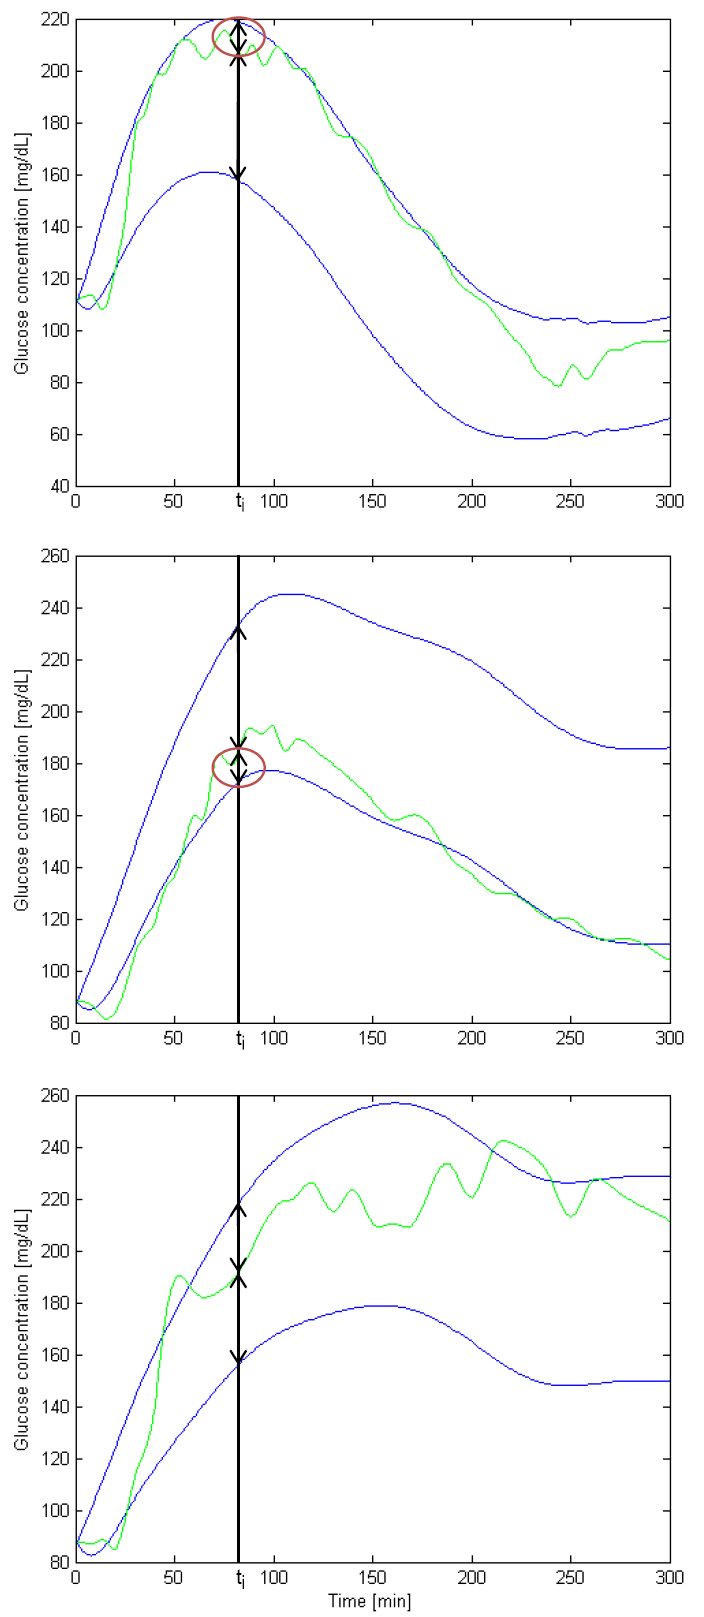
\epsfig{file=Figures/overstimation.png, width=0.5\textwidth}\caption{Graphic description of the envelope fitness index. Three postprandial periods are displayed for both YSI data (green) and glucose envelopes (blue). Distances of the data to the envelope are displayed, and the minimum distances to the upper and lower bounds are highlighted. The average distance along time defines the envelope width fitness to data.}
\label{fig:overstimation}
\end{figure}

All measures listed above have to be considered simultaneously when evaluating an identification experiment. An identification with low predicted samples does not mean a bad identification result if it simultaneously presents a very low relative error. Similarly, an identification with many predicted samples (on the validation day) but poor envelope fitness (on the identification days) may correspond to a trivial solution of the identification problem.

Mean, median, standard deviation and maximum/minimum values of the above measures for all the patients are reported. All significances were calculated using non-parametric Fisher's resampling test.

\section{Validation Results}
\label{sec:IdentificationFromReferenceGlucose2}

%Although a 12 patients experiment is hardly enough to draw conclusions on the general type 1 diabetic population, we believe useful information can be drawn from these results regarding %management of intra-patient variability in the challenging problem of model identification in type 1 diabetes.

The different evaluation measures for the cross-validation study are reported in Table \ref{tab:results2scenarios} for identification and validation days. Evaluations on the identification days are used to test the fitting quality, while the evaluation on the validation set is a good representation of the predictability of the method and thus the overall performance of the identifications. The identified interval and real-valued parameters are reported in Table \ref{tab:identifiedparam}. Mean and median values for the midpoint and width of the intervals are shown, for the sake of simplicity. Median values are a good estimation of the magnitude of the identification results as they better filter outlier and are better estimators of the distribution expectancy for skewed distributions, but mean values of the evaluation measurements are useful for comparison between scenarios and datasets.

\begin{sidewaystable}[hbtp]
	\centering
	\begin{tabular}{| c | c | c | c | c | c | c | c |}
	\multicolumn{1}{c}{Scenario} & \multicolumn{1}{c}{} & \multicolumn{1}{c}{Width} & \multicolumn{1}{c}{Prediction} & \multicolumn{1}{c}{MARDout} & \multicolumn{1}{c}{MARDtot} & \multicolumn{1}{c}{gMARDout} & \multicolumn{1}{c}{gMARDtot} \\
	\multicolumn{1}{c}{} & \multicolumn{1}{c}{} & \multicolumn{1}{c}{[mg/dL]} & \multicolumn{1}{c}{[\%]} & \multicolumn{1}{c}{[\%]} & \multicolumn{1}{c}{[\%]} & \multicolumn{1}{c}{[\%]} & \multicolumn{1}{c}{[\%]} \\
	\hline
	\multicolumn{8}{c}{Identification days}\\
	\hline
	\multirow{4}{*}{1} & mean & 87.7 & 77.9 & 5.79 & 1.22 & 5.92 & 1.26 \\
	\cline{2-8}
  & SD & 39 & 7.2 & 6.1 & 1.07 & 6.11 & 1.09 \\
	\cline{2-8} 
	& median & 81.2 & 78.9 & 4 & 0.92 & 4.11 & 0.94 \\
	\cline{2-8} 
	& max/min & 187.9/40.4 & 92.2/63.6 & 32.14/1.37 & 4.84/0.24 & 32.16/1.38 & 4.85/0.24 \\
	\hline 
	\multirow{4}{*}{2} & mean & 94.8 & 78.4 & 6.56 & 1.35 & 6.7 & 1.38 \\
	\cline{2-8} 
  & SD & 42.5 & 6.8 & 9.01 & 1.64 & 9.01 & 1.64 \\
	\cline{2-8} 
	& median & 89.9 & 78.1 & 3.9 & 0.85 & 4.08 & 0.88 \\
	\cline{2-8} 
	& max/min & 218.3/41.2 & 93.4/64.7 & 48.84/1.67 & 7.89/0.25 & 48.87/1.67 & 7.89/0.25 \\
	\hline
	\multicolumn{8}{c}{Validation days}\\
	\hline
	\multirow{4}{*}{1} & mean & 78.8 & 53.5 & 12.23 & 7.61 & 13.46 & 8.51 \\
	\cline{2-8}
  & SD & 38.4 & 30.1 & 8.83 & 7.88 & 10.62 & 9.72 \\
	\cline{2-8}
	& median & 66.4 & 52.8 & 11.22 & 5.56 & 11.97 & 5.59 \\
	\cline{2-8}
	& max/min & 205.1/29.3 & 100/0.7 & 32.93/0 & 30.41/0 & 48.49/0 & 44.77/0 \\
	\hline 
	\multirow{4}{*}{2} & mean & 83.9 & 54.9 & 12.66 & 8.09 & 13.91 & 8.95 \\
	\cline{2-8} 
  & SD & 40.8 & 31.9 & 10.3 & 9.06 & 11.69 & 10.43 \\
	\cline{2-8} 
	& median & 79.1 & 57 & 9.65 & 5.45 & 12.14 & 5.84 \\
	\cline{2-8} 
	& max/min & 222/34.6 & 100/0.3 & 37.87/0 & 31.19/0 & 43.42/0 & 39.57/0 \\
  \hline 
	\end{tabular}
\caption{Results for both scenarios for the 3 identification days with all the possible permutations, and the validation days.}
\label{tab:results2scenarios}
\end{sidewaystable}

\begin{sidewaystable}[hbtp]
	\centering
	\begin{tabular}{| c | c | c | c | c | c | c | c |}
	
	\cline{4-8}
	\multicolumn{3}{c|}{\textbf{Interval}} & $S_{IT} \times 10^{-3}$ & $S_{ID} \times 10^{-4}$ & $S_{IE} \times 10^{-2}$ & $k_{12} \times 10^{-2}$ & \multirow{2}{*}{$\alpha$} \\
	\multicolumn{3}{c|}{\textbf{parameters}} & $\left[mU/min\cdot L\right]$ & $\left[mU/min\cdot L\right]$ & $\left[mU/min\cdot L\right]$ & $\left[min^{-1}\right]$ & \\
	\hline
	\multirow{4}{*}{Scenario 1} & Mid & mean & 5.05 & 6.08 & 4.43 & 6.43 & 1.12 \\
	& point & SD & 1.32 & 3.06 & 2.11 & 2.45 & 0.4 \\
	\cline{2-8}
	& \multirow{2}{*}{Width} & mean & 2.39 & 0.05 & 0.45 & 1.16 & 0.02 \\
	& & SD & 1.62 & 0.25 & 0.9 & 2.01 & 0.08 \\
	\hline
	\multirow{4}{*}{Scenario 2} & Mid & mean & 5.04 & 6.05 & 4.12 & 6.72 & \multirow{4}{*}{fixed} \\
	& point & SD & 1.24 & 2.83 & 1.92 & 2.57 & \\
	\cline{2-7}
	& \multirow{2}{*}{Width} & mean & 2.86 & 0.04 & 0.39 & 1.09 & \\
	& & SD & 1.53 & 0.2 & 0.77 & 2.16 & \\
	\hline
	\multicolumn{3}{|c|}{Nominal value} & 5.12 & 8.2 & 5.2 & 6.6 & 1 \\
	\hline
	\hline
  \multicolumn{3}{|c|}{\textbf{Real-valued parameters}} & $t_{maxG40} [min]$ & $t_{maxG100} [min]$ & \multicolumn{1}{c}{} & \multicolumn{1}{c}{} & \multicolumn{1}{c}{} \\
	\cline{1-5}
	\multirow{2}{*}{Scenario 1} & \multicolumn{2}{c|}{mean} & 85.1 & 98.8 & \multicolumn{1}{c}{} & \multicolumn{1}{c}{} & \multicolumn{1}{c}{} \\
	 & \multicolumn{2}{|c|}{SD} & 68.5 & 31.4 & \multicolumn{1}{c}{} & \multicolumn{1}{c}{} & \multicolumn{1}{c}{} \\
	\cline{1-5}
	\multirow{2}{*}{Scenario 2} & \multicolumn{2}{c|}{mean} & 87.2 & 99.2 & \multicolumn{1}{c}{} & \multicolumn{1}{c}{} & \multicolumn{1}{c}{} \\
	 & \multicolumn{2}{|c|}{SD} & 66.7 & 39.8 & \multicolumn{1}{c}{} & \multicolumn{1}{c}{} & \multicolumn{1}{c}{} \\
	\cline{1-5} 
	\multicolumn{3}{|c|}{Nominal value} & 40 & 40 & \multicolumn{1}{c}{} & \multicolumn{1}{c}{} & \multicolumn{1}{c}{} \\
	\cline{1-5} 
	\end{tabular}
	
\caption{Identified parameters for both scenarios. Nominal values were extracted from \cite{hovorka2004nonlinear}.}
\label{tab:identifiedparam}
\end{sidewaystable}

The mean value of the envelope fitness function for scenario 1 was 19.35 mg/dL (median 14.59 mg/dL) while for scenario 2 was 21.7 mg/dL (median 15.98 mg/dL). Fitness value per patient and scenario is reported in Figure \ref{fig:fitnessperpatient}. Patient 12 presents very poor envelope fitness value on both scenarios, and can be considered as an outlier.

\begin{figure}[hbtp]
\centering
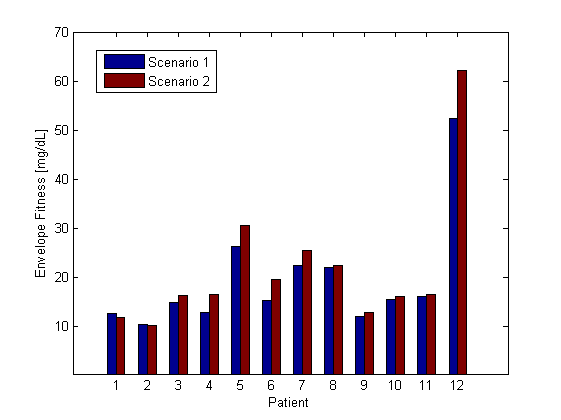
\epsfig{file=Figures/fitnessperpatient.png, width=\textwidth}\caption{Envelope fitness for every patient and scenario.}
\label{fig:fitnessperpatient}
\end{figure}

Analyzing the results in Table \ref{tab:results2scenarios} it can be observed that envelope widths for the three identification days were greater than those shown in the validation day (scenario 1: 87.7 vs. 78.8 mg/dL, p<0.005; scenario 2: 94.8 vs. 83.9 mg/dL, p<0.005). Identified widths were large, but the uncertainty registered resembled the observed intra-patient variability, given that the envelope fitness measure on both scenarios was good in average (14.59 vs. 15.98 mg/dL). This yields to an expectancy of the maximum separation of the prediction boundaries from the actual data in accordance to current criteria for glucose measuring devices accuracy. This result is valid throughout all the postprandial periods, implying that the method accurately fits the provided data even though prediction bands are wide. Besides, errors for validation days were (as expected) larger than those for identification days for both scenarios \ref{tab:results2scenarios}. 

There were no great differences in the overall performance comparing validation results between scenarios. No statistically significant difference in the prediction error was found (7.61 vs. 8.09, p=0.237) despite smaller envelope maximum widths in favor of scenario 1 (78.79 vs. 83.9, p<0.005). This is so because maximum width tends to happen at the end of the postprandial period when data are more likely to be enclosed (contributing with zero error to the MARD), not having an impact in the overall prediction error. Nevertheless, the difference in the envelope maximum width (5.11 mg/dL) was not considered clinically relevant. 

This equivalence between scenarios may suggest identifiability issues (as commonly observed in identification studies) and difficulties to properly detect the physiological source of uncertainty due to the nature of data used. Indeed, uncertainty sources were found in repeated patterns all across the identifications when looking at the identified parameters (see Table \ref{tab:identifiedparam}). In this regard, Table \ref{tab:uncertaintyscenarios} shows the number of identifications for each scenario that showed uncertainty in each of the interval parameters considered. If both limits of the interval parameter were identified to be the same, that parameter was considered real-valued and no uncertainty was assumed to exist in that case. 

\begin{table}[hbtp]
	\centering
	\begin{tabular}{ c | c  c  c  c  c }
   & $S_{IT}$ & $S_{ID}$ & $S_{IE}$ & $k_{12}$ & $\alpha$ \\
	\hline
	Scenario 1 & 95.8\% & 4.2\% & 33.3\% & 41.7\% & 6.3\% \\
	Scenario 2 & 93.8\% & 4.2\% & 29.2\% & 35.4\% & fixed \\
	\hline
	\end{tabular}
\caption{Percentage of identifications in which each parameter presented uncertainty.}
\label{tab:uncertaintyscenarios}
\end{table}

Values in Table \ref{tab:identifiedparam} are related to the widths of the intervals in Table \ref{tab:uncertaintyscenarios}. If the interval is identified in many occasions as a real-valued parameter, the average width of that parameter will be very low. Parameters $S_{IT}$ and $k_{12}$ were the most uncertain parameters in both scenarios, which are interestingly both related to glucose transport between plasma and interstitial fluid. However, the gastrointestinal system contributed to uncertainty for scenario 1 only in 6\% of the trials despite the variability expected a priori according to tracer studies. This may be due, at least in part, to the consideration of two different $t_{maxG}$ parameters dependent on the meal size, which were found statistically significantly different for both scenarios (see Table \ref{tab:identifiedparam}), and the few instances available of repeated meals during cross-validation (only two of the days used for each identification permutation were subject to pure gastrointestinal variability, i.e., the two days with identical meal input). This resulted in small widths for the common parameter $\alpha$. Richer (more repeated meals, tracer studies) data would most probably lead to larger variability in the gastrointestinal system. This is considered a limitation of the current data and further investigation is required. However, prediction ability of the method was demonstrated and no technical limitations exist should tracer data or longer time series be available.

As an illustration, identification results for two patients are shown in figures \ref{fig:pacient2} and \ref{fig:pacient9}, for each identification-validation day permutation. Even though four simulated postprandial periods are displayed per identification, the simulations were not consecutive. Every day was simulated separately considering steady-state initial conditions in order to account for the pre-prandial stabilization period of the patients. Then the simulation profiles were concatenated for better illustration of the overall identification performance. Results are shown for scenario 1, although both scenarios reported very similar outcomes.

\begin{figure}[hbtp]
\centering
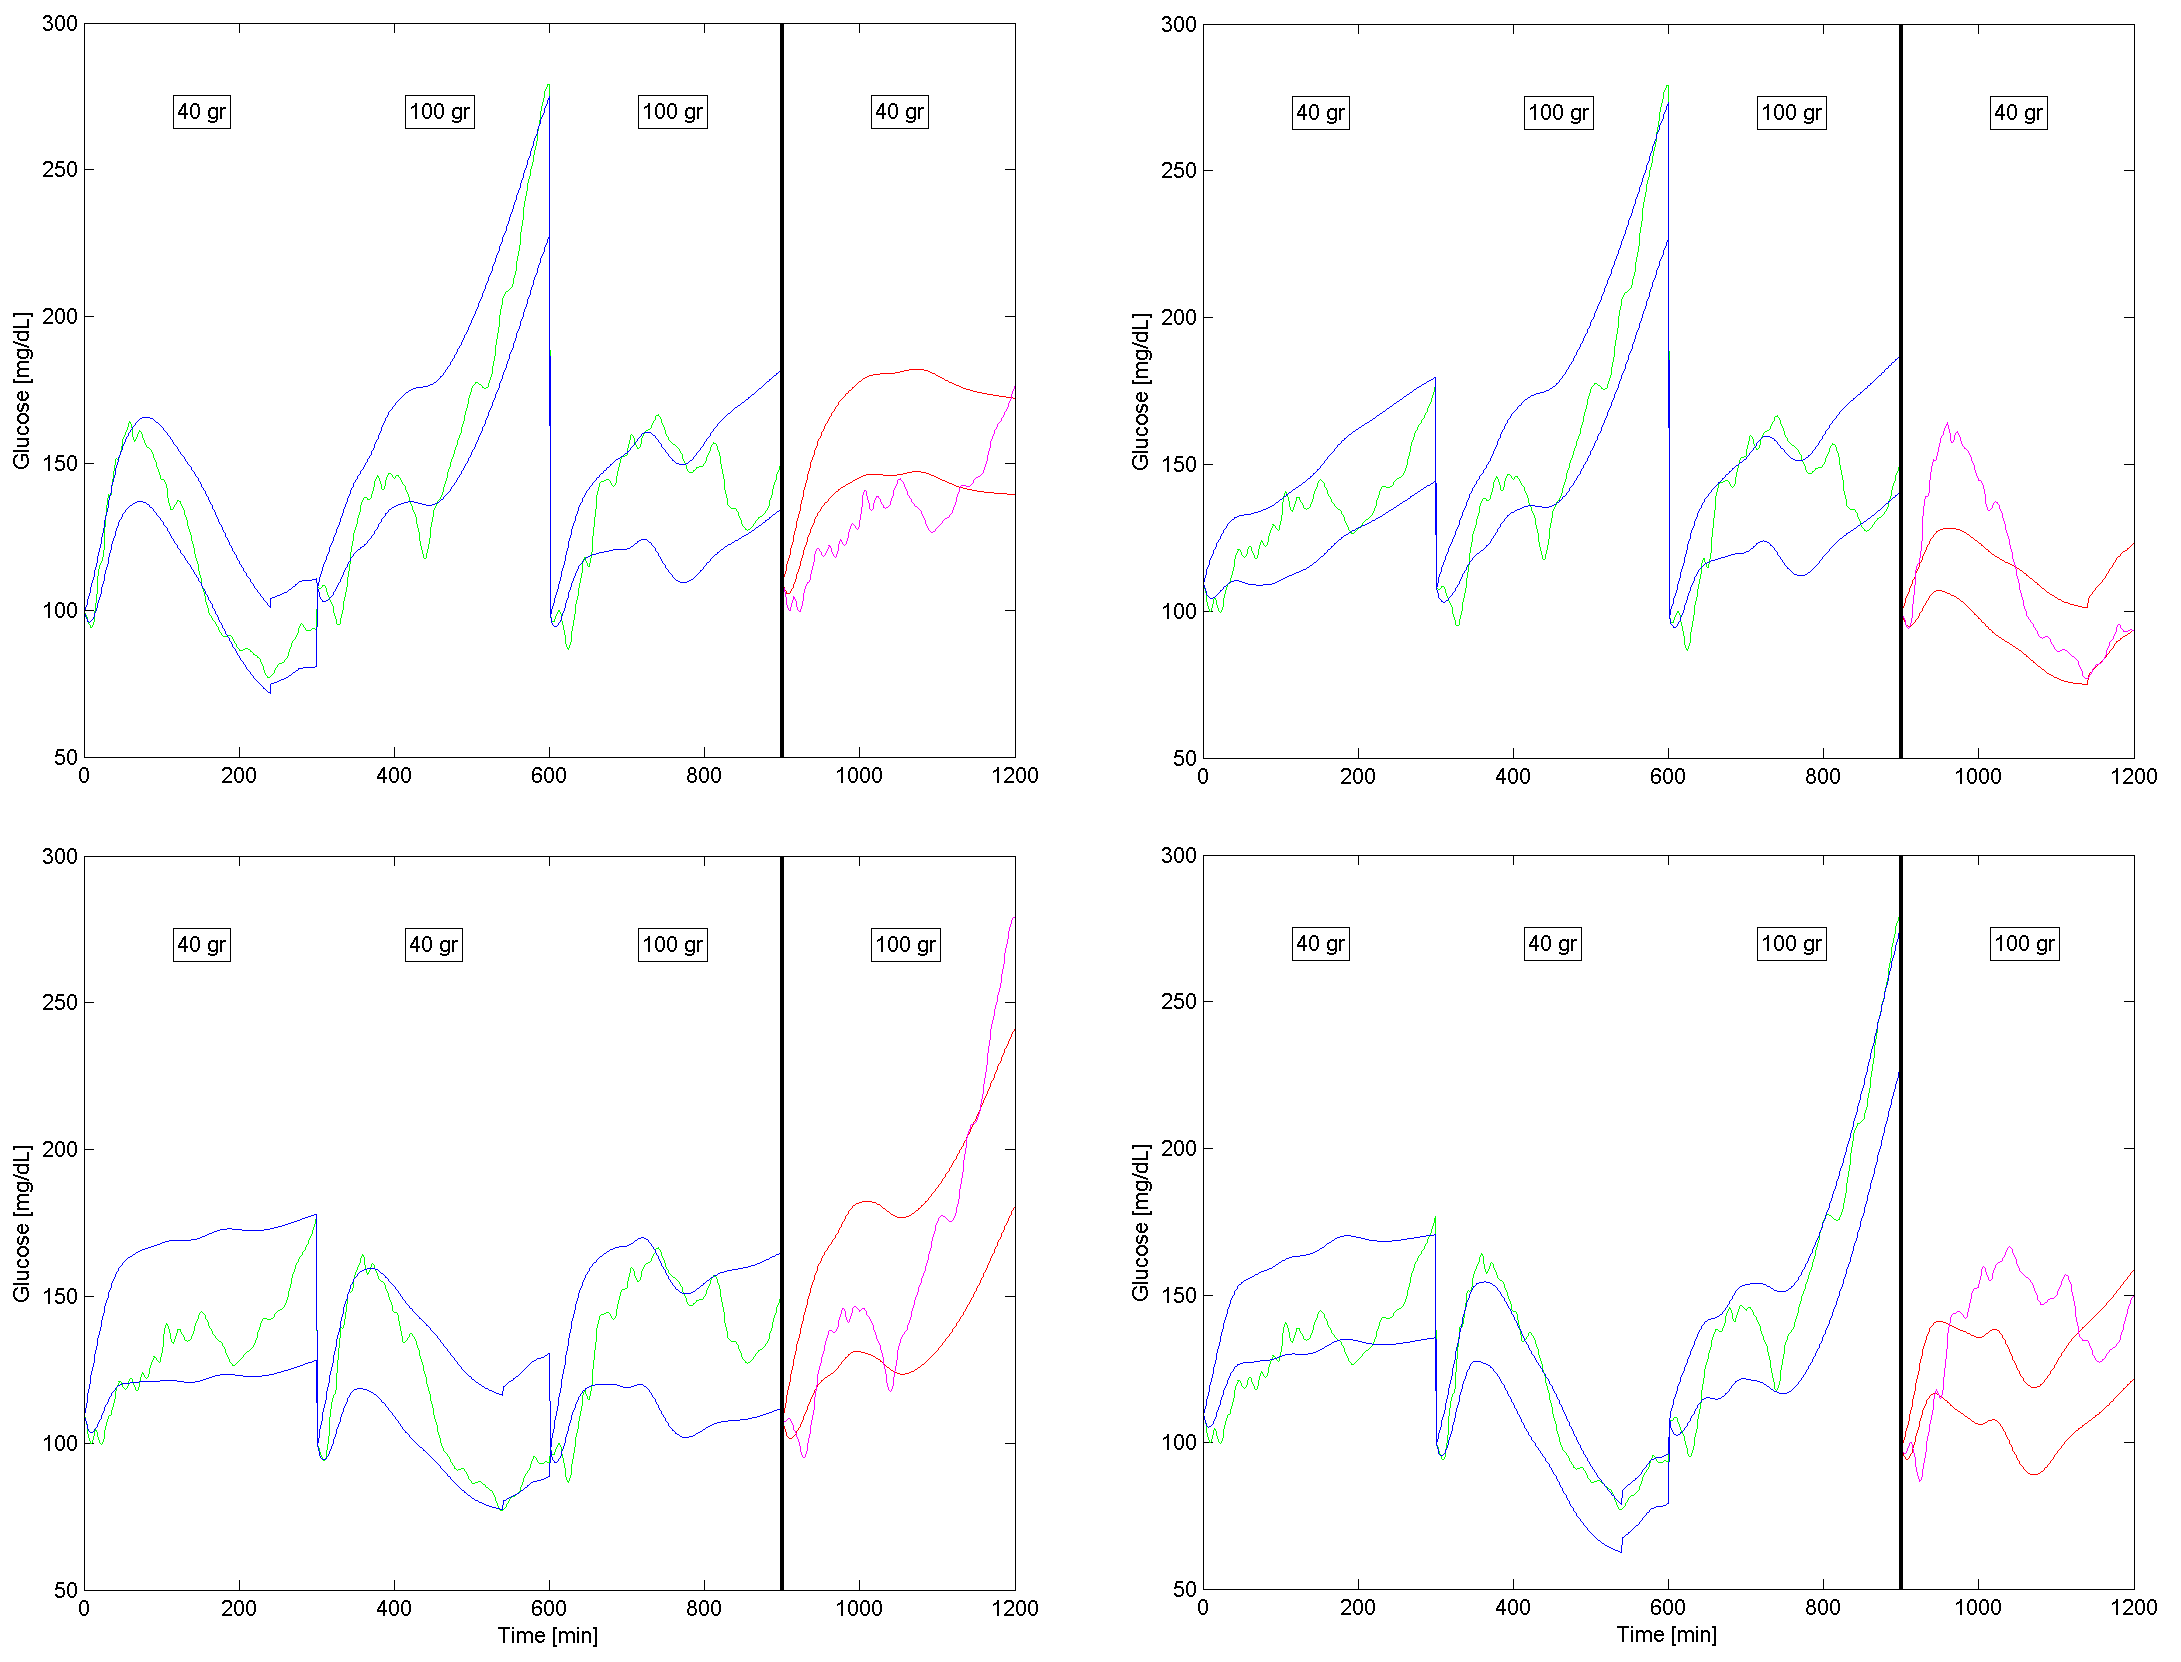
\epsfig{file=Figures/pacient2.png, width=\textwidth}\caption{Patient 2 identification and validation results for the scenario 1. Day 1 validation is shown top left. Top Right graph shows validation for day 2. Bottom left validates day 3. Bottom right shows validation for day 4.}
\label{fig:pacient2}
\end{figure}

Figure \ref{fig:pacient2} (patient 2) poses an example of an average patient's identification outcome. Results correspond to scenario 1 because of physiological soundness, although both scenarios reported very similar outcomes. For the first permutation (top left), validation was not successful (MARDtot = 7.39\%). Most of the postprandial data was overestimated, even though 5-hour glucose value was well captured. Though, in clinical terms, the identification implied no danger for the patient (gMARDtot = 7.39\%), since the clinical index was exactly the same than the prediction error. For the second permutation (top right), dynamics were modeled correctly, but postprandial peak was greatly underestimated (MARDtot = 6.03\%), and the effect of glucose infusion in the last hour to avoid hypoglycemia was overestimated. Since no dangerous zones were left unmodelled, clinical validation was also successful (gMARDtot = 6.03\%). Third permutation (bottom left) captured perfectly the dynamics of the postprandial period, even though no similar behaviors are observed in the identification days, only leaving out of prediction the last part of the 5-hour period (MARDtot = 2.29\%). However, clinical validation was not so good in this case, with gMARDtot = 3.58\% due to the last part of the simulation not being able to follow the rapid rise of glucose, missing thus the hyperglycemia risk. Fourth permutation (bottom right) showed some not predicted samples (MARDtot = 9.18\%), but no clinical risk was involved (MARDtot = 9.2\%).

\begin{figure}[hbtp]
\centering
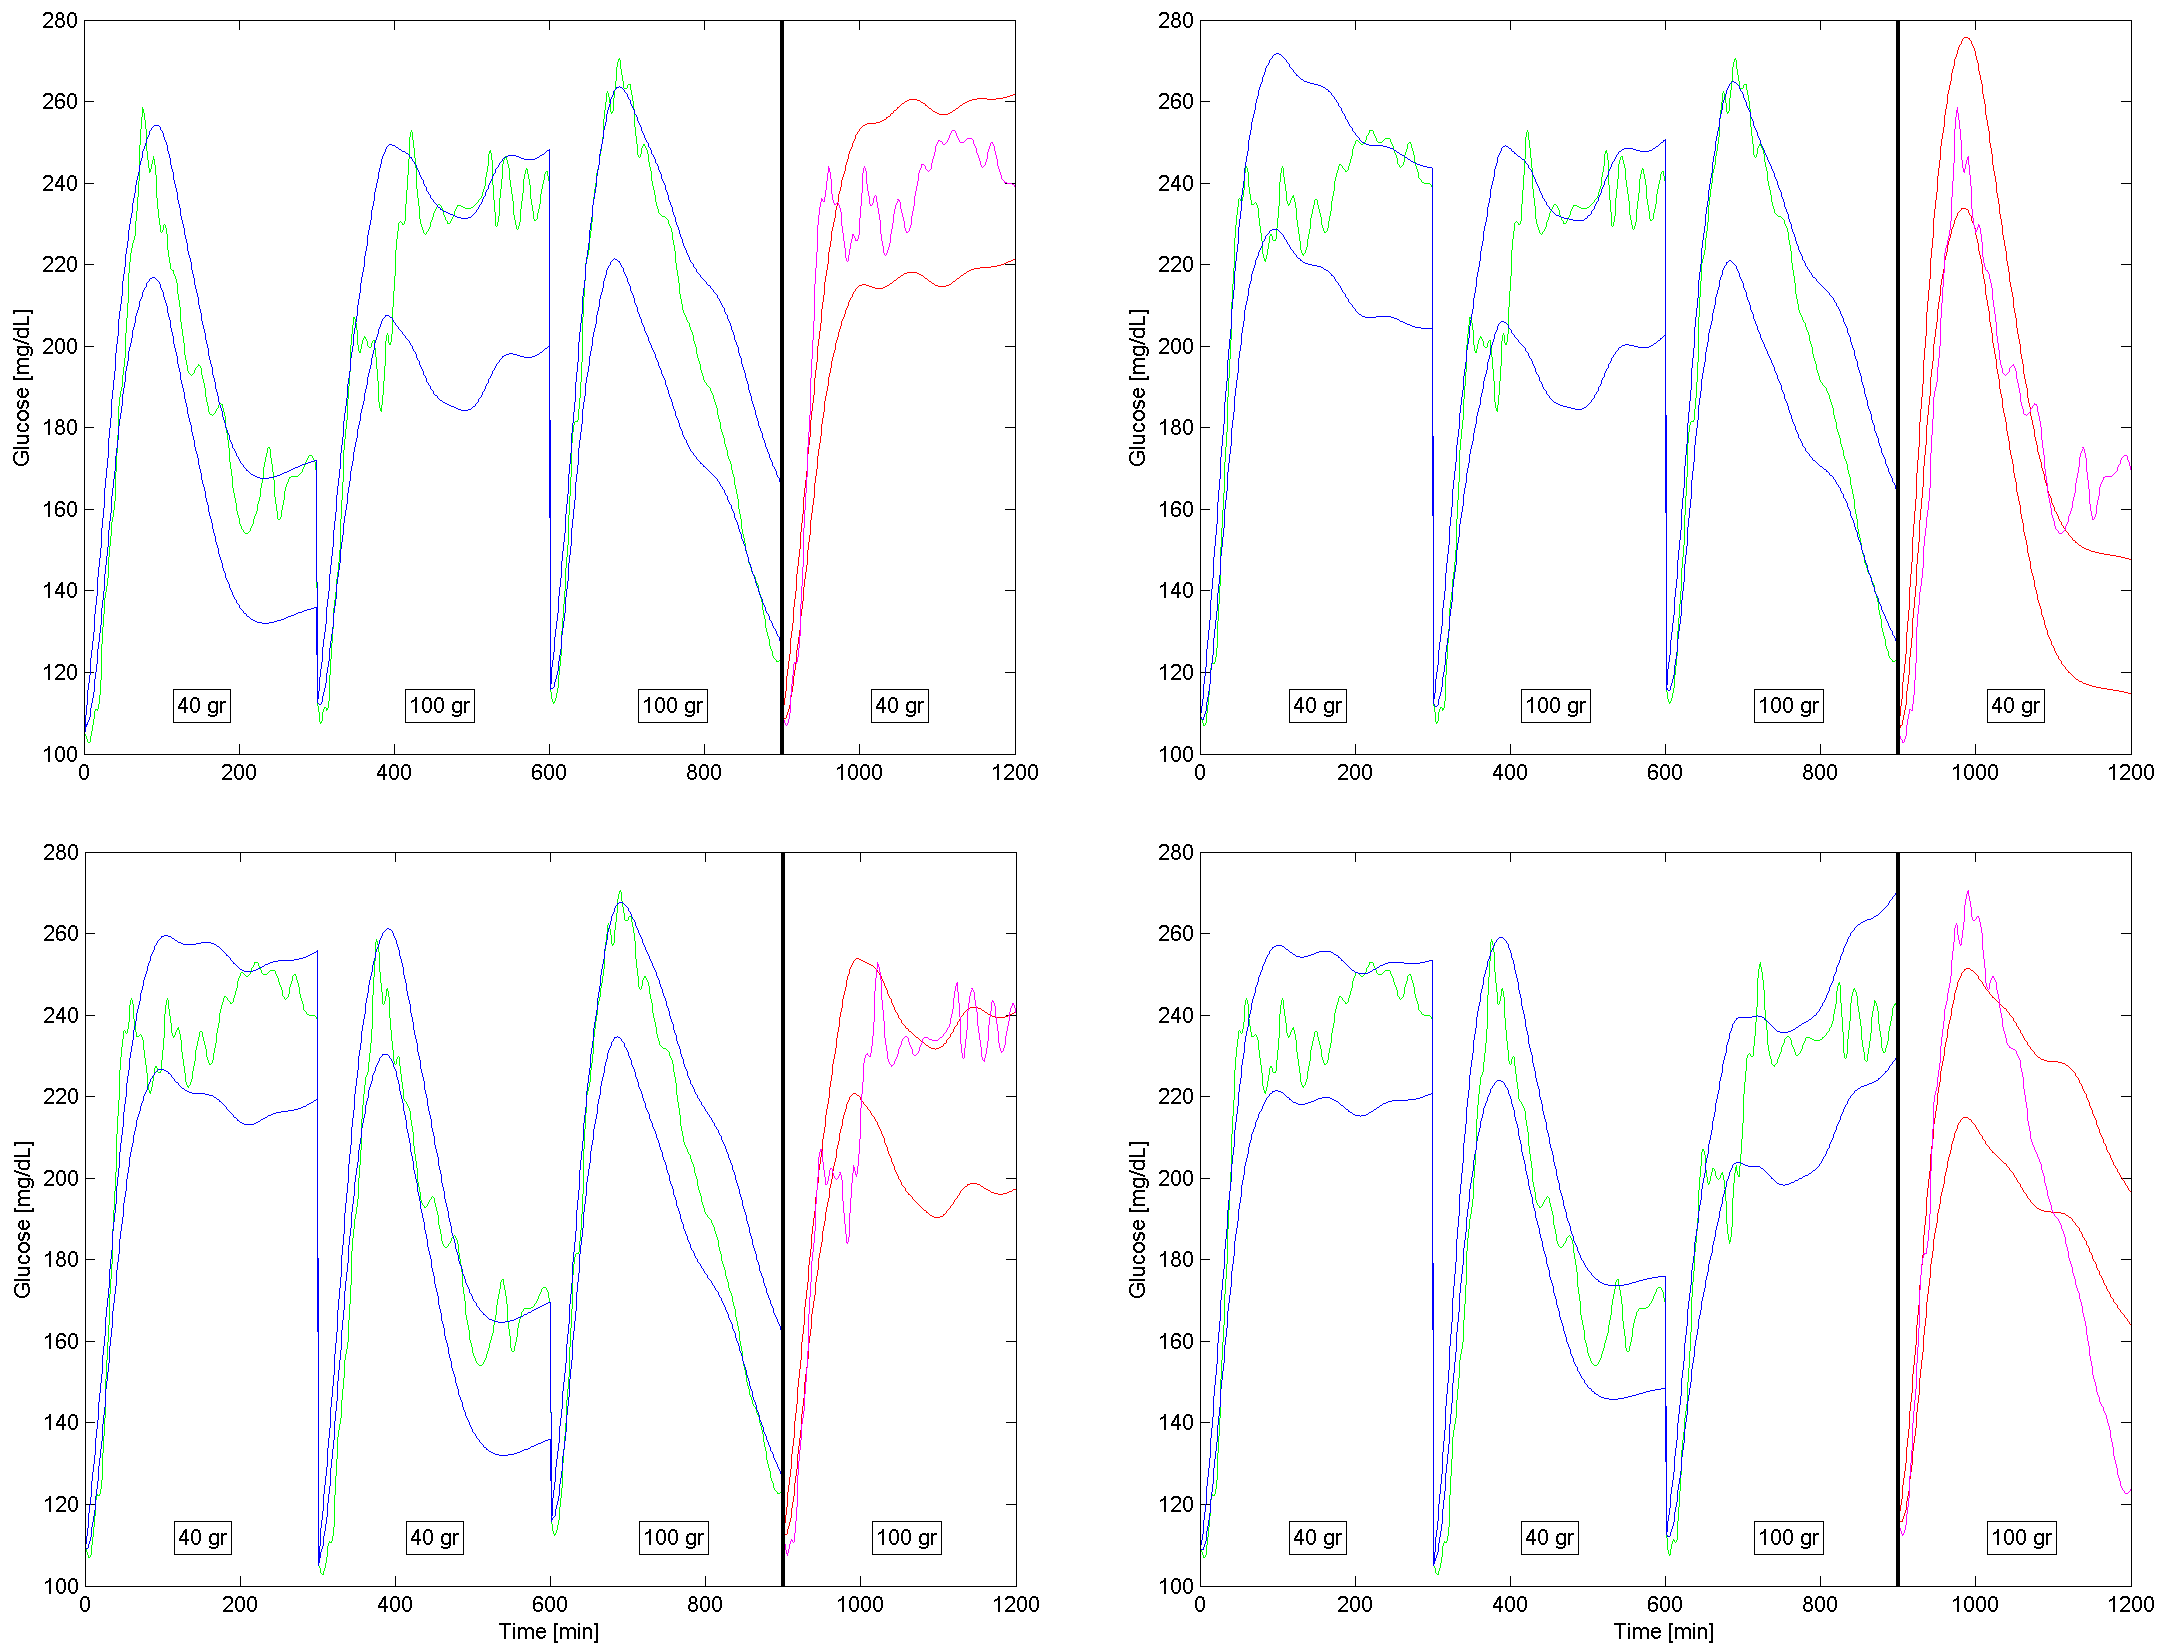
\epsfig{file=Figures/pacient9.png, width=\textwidth}\caption{Patient 9 identification and validation results for the scenario 1. Day 1 validation is shown top left. Top Right graph shows validation for day 2. Bottom left validates day 3. Bottom right shows validation for day 4.}
\label{fig:pacient9}
\end{figure}

Figure \ref{fig:pacient9} presents a case of a better identification, corresponding to patient 9. Day 1 prediction envelope (top left) covered almost all the blood glucose samples, and the overall error was very small (MARDtot = 1.03\%). Clinical error was not much higher (gMARDtot = 1.8\%) in this validation because most part of the postprandial period is spent in hyperglycemic region, and the model fails to predict a small part of it, although with very small error. The patient was well predicted when validating with day 2 (top right) except in the 5-hour horizon (MARDtot = 4.93\%). Validation was also really good for day 3 (bottom left), with a MARDtot of 1.88\%. Dynamics were well captured when validating with day 4 (bottom right), with some lack of predictability from 3 hours onward in the postprandial period (MARDtot = 6.88\%). As happened with the first day, the clinical error is a little bit higher because the model fails to predict the hyperglycemic peak, but with very small error. As result, the patient was successfully identified for every permutation, capturing the dynamics of the patient independently of the days used for identification for an average envelope fitness function value of about 11.87 mg/dL (see Figure \ref{fig:overstimation}).

\section{Best-case permutation}
\label{sec:BestCasePermutation}

\begin{figure}[hbtp]
\centering
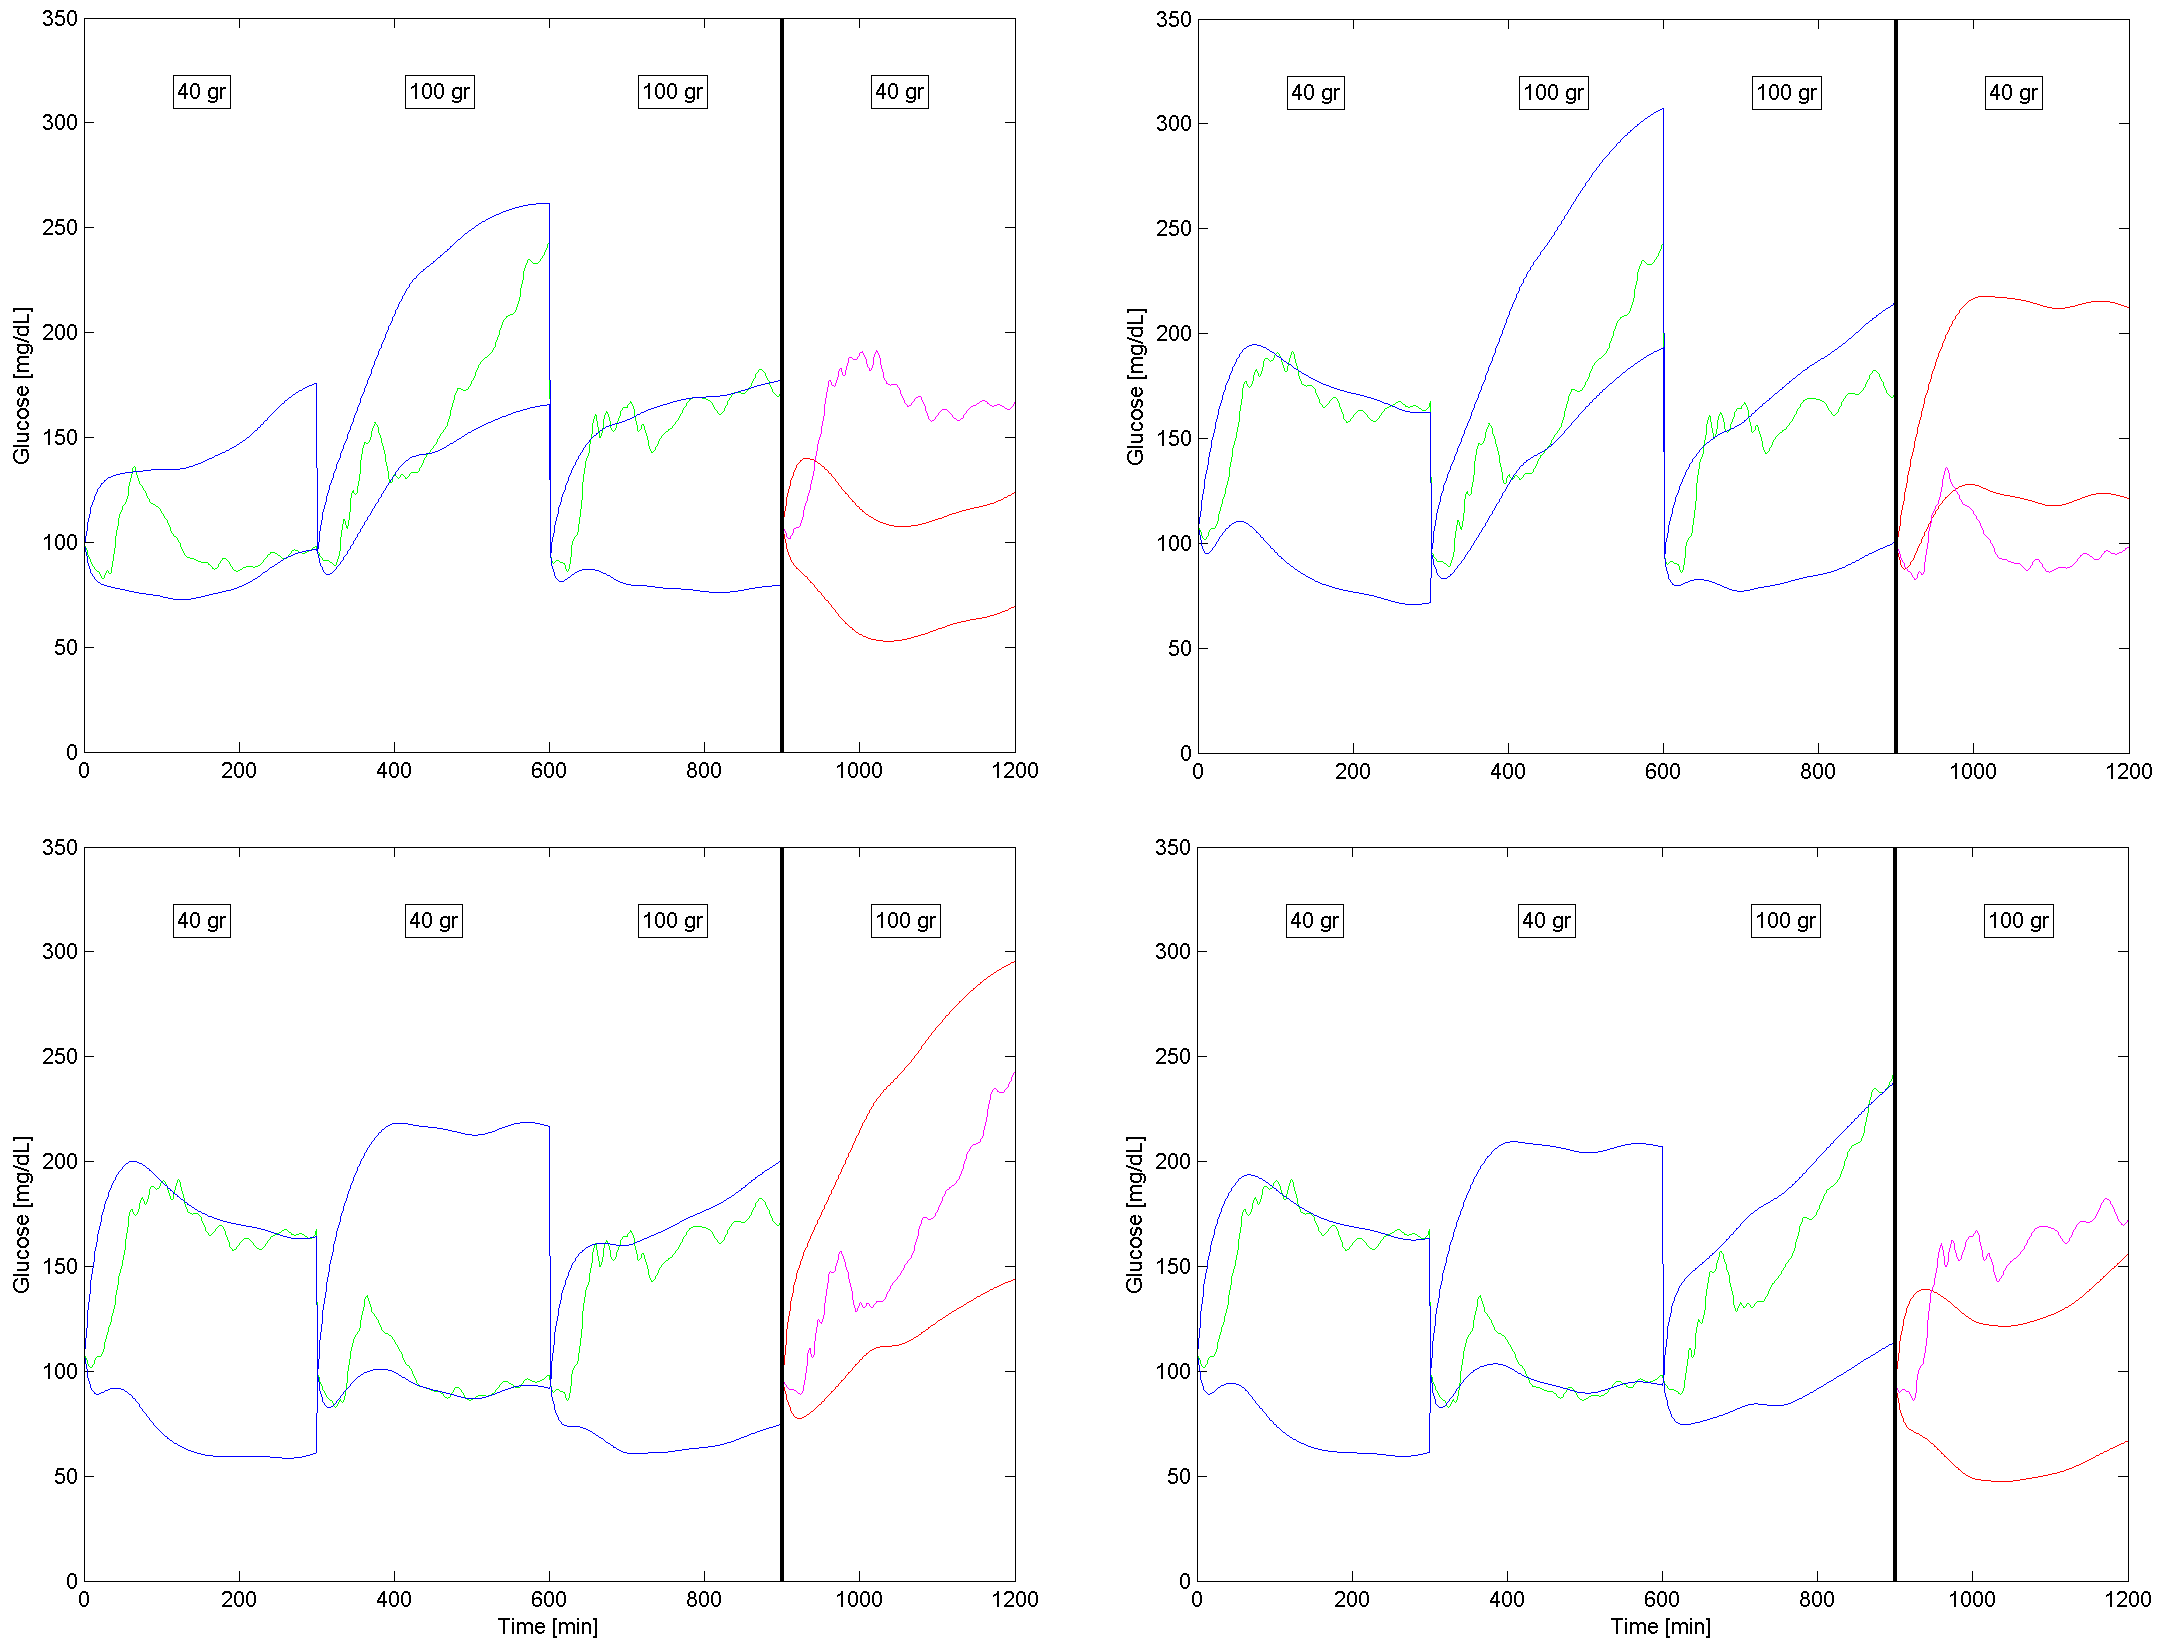
\epsfig{file=Figures/pacient11.png, width=\textwidth}\caption{Patient 11 identification and validation results for the scenario 1. Day 1 validation is shown top left. Top Right graph shows validation for day 2. Bottom left validates day 3. Bottom right shows validation for day 4.}
\label{fig:pacient11}
\end{figure}

Figure \ref{fig:pacient11} represents a patient with very good prediction for only one validation day, corresponding to patient 11. As with the other examples, results are shown for scenario 1, although both scenarios reported very similar outcomes. This is most illustrative case for the best case of a particular patient. We can see how only when days 1, 2 and 4 were used for identification (bottom left), dynamics of the validation day was well characterized. In all the other cases, the identification was unsuccessful. Envelope width for the best-case day was also wider than in the other cases (without width overestimation). This fact leads to think that variability of this particular patient showed its maximum for that particular permutation of monitoring days. Maximization of predictability is then straightforward if interval model identification works best when maximum variability is present in the data: the more days available the higher the variability, thus the better the prediction. 

As it may be observed from patient 11, validation results are dependent on the permutation considered due to the different representativeness of the identification days with regard to the exhibited intra-patient variability. In the general case, out of the four permutations of the identification, usually one or two of them presented a very small error, while the rest did not capture correctly the behavior of the patient mainly due to lack of representativeness of the identification data with regard to the exhibited intra-patient variability. Indeed, it cannot be expected to predict a behavior in the validation day significantly different than the ones present in the identification data. The inclusion of more days for identification would reduce this problem. In this regard, a best-case permutation was defined as the permutation with minimum clinical error gMARDtot, thus minimizing both the fitting error and the danger to the patient. When two of the permutations showed similar results, the solution with the minimum width was considered the best one. Table \ref{tab:resultsbestcase} shows the evaluation measures for the validation days considering the best-case permutation. Mean envelope fitness for the best cases in scenario 1 was 19.87 mg/dL (median 15.55 mg/dL), and for scenario 2 was 26.74 mg/dL (median 19.98 mg/dL).

\begin{sidewaystable}[hbtp]
	\centering
	\begin{tabular}{| c | c | c | c | c | c | c | c | c |}
	\hline
	Scenario & \multicolumn{4}{|c|}{1} & \multicolumn{4}{|c|}{2} \\
	\hline
	& Mean & SD & median & max/min & Mean & SD & median & max/min \\
	\hline
	Width & \multirow{2}{*}{104.6} & \multirow{2}{*}{51.1} & \multirow{2}{*}{94.3} & \multirow{2}{*}{201.1/42.5} & \multirow{2}{*}{103.8} & \multirow{2}{*}{43.6} & \multirow{2}{*}{101.3} & \multirow{2}{*}{179.2/43.5} \\[0pt]
	[mg/dL] & & & & & & & & \\
	\hline
	Prediction & \multirow{2}{*}{87.3} & \multirow{2}{*}{17.6} & \multirow{2}{*}{97.3} & \multirow{2}{*}{100/52.3} & \multirow{2}{*}{87.1} & \multirow{2}{*}{18.4} & \multirow{2}{*}{96.8} & \multirow{2}{*}{100/45.3} \\[0pt]
	[\%] & & & & & & & & \\
	\hline	
	MARDout & \multirow{2}{*}{4.38} & \multirow{2}{*}{5.78} & \multirow{2}{*}{1.51} & \multirow{2}{*}{17.81/0} & \multirow{2}{*}{3.32} & \multirow{2}{*}{4.41} & \multirow{2}{*}{0.87} & \multirow{2}{*}{13.17/0} \\[0pt]
	[\%] & & & & & & & & \\
	\hline
	MARDtot & \multirow{2}{*}{1.24} & \multirow{2}{*}{2.43} & \multirow{2}{*}{0.03} & \multirow{2}{*}{8.49/0} & \multirow{2}{*}{0.8} & \multirow{2}{*}{1.18} & \multirow{2}{*}{0.03} & \multirow{2}{*}{3.38/0} \\[0pt]
	[\%] & & & & & & & & \\
	\hline
	gMARDout & \multirow{2}{*}{5.08} & \multirow{2}{*}{6.27} & \multirow{2}{*}{1.51} & \multirow{2}{*}{17.81/0} & \multirow{2}{*}{4.24} & \multirow{2}{*}{5.79} & \multirow{2}{*}{0.87} & \multirow{2}{*}{15.94/0} \\[0pt]
	[\%] & & & & & & & & \\
	\hline
	gMARDtot & \multirow{2}{*}{1.41} & \multirow{2}{*}{2.51} & \multirow{2}{*}{0.03} & \multirow{2}{*}{8.49/0} & \multirow{2}{*}{1.06} & \multirow{2}{*}{1.72} & \multirow{2}{*}{0.03} & \multirow{2}{*}{5.63/0} \\[0pt]
	[\%] & & & & & & & & \\
	\hline
	\end{tabular}
\caption{Results for both scenarios for the validation days of the best case permutation.}
\label{tab:resultsbestcase}
\end{sidewaystable}

Table \ref{tab:resultsbestcase} shows the evaluation metrics for the best-case permutation for each patient. As expected, errors for the validation days were significantly smaller for the best cases with respect to results in Table \ref{tab:results2scenarios} (scenario 1: 1.24 vs.7.61 \% p<0.005; scenario 2: 0.8 vs. 8.09 \%, p<0.005). Widths were significantly larger for scenario 1 (104.6 vs.78.8 mg/dL, p=0.034) but not significantly larger for scenario 2 (103.8 vs. 83.8 mg/dL, p=0.075), although we assume this lack of significance is due to the small sample size of 12 patients, and should the number of patients be larger, the difference in widths is expected to increase. This increment in the width was due to the increment of variability present in the identification data, improving representativeness of the patient's behavior, and thus validation results. No additional envelope width overestimation was found for scenario 1 (mean/median:  19.87/15.55 mg/dL versus 19.35/14.59 mg/dL for the whole data set). It was not so for scenario 2 (mean/median:  26.74/19.98 mg/dL versus 21.70/15.98 mg/dL ) which compensated the non-physiological consideration of lack of variability in the gastrointestinal model with envelope width overestimation. Indeed, median Predictions value was over 95\% (mean value over 85\%) for both scenarios. This implied errors virtually equal to zero, and complete coverage of the validation data. No difference in the width between the scenarios was found (see Table \ref{tab:resultsbestcase}). However, the observed envelope width overestimation for scenario 2 leads to the conclusion that scenario 1 better represents intra-patient variability without incurring in model overfitting.

Finally, comparing Tables \ref{tab:results2scenarios} and \ref{tab:resultsbestcase}, clinical indexes were statistically significantly larger than their pure error counterparts, both for the whole dataset (scenario 1: 8.51 vs.7.61 \%, p<0.005; scenario 2: 8.95 vs. 8.09 \%, p<0.005) and for the best-case permutations (scenario 1: 1.41 vs. 1.24, p<0.005; scenario 2: 1.06 vs. 0.8, p<0.005). However, differences between gMARDtot and MARDtot were reduced from approximately 1\% for the whole dataset to approximately 0.2\% (corresponding to underestimated mild hyperglycemia according to \cite{del2012glucose}, Fig. 2) for the best-case permutation. Hypoglycemia risk was not at stake.

\section{Discussion}
\label{sec:Discussionip}
	
Identification from experimental data supposes a great challenge. The case exposed in this chapter is the simplest situation of identification with real patient's data the author was aware of, and yet identification procedures turned out very complex. A complete identification study with implicit consideration of uncertainty in the system has been presented. Identification was performed using a hybrid cost index minimizing both the envelope width of the interval prediction model so that uncertainty is minimal, and fitting error to the data. Only the endogenous and gastrointestinal models where considered in this chapter, as an in-patient identification study.

Identification of the 12 patients showed good prediction capabilities in average and especially when the maximum variability, or uncertainty for that particular patient, was represented in the identification days (best-case permutation). A larger number of monitoring days of the same patient would increase the probability of extreme variations of the metabolism of the patient, thus easing the identification and increasing the predictability of the data. A limitation of the study was precisely the nature of the data that prevented to draw conclusions on the source of the identified uncertainty. Contrary to tracer studies, the results here exposed did not show significant uncertainty in the gastrointestinal system compared to the insulin and endogenous subsystem, most probably due to data limitations. 

The existence of best-case permutation and the possibility of predicting the behavior of the patient using this combination is the most important contribution of this chapter, and one of the main findings of the thesis. Although it is well known that patient variability in diabetes is very high, this work is the first successful identification process performed on real data including variability. The best-case permutation for each patient is still impossible to predict, and apparently appears at random in the dataset used for this chapter. Further work can be done on investigating the characteristics of the patient on the days of maximum variability, using for example pattern search on physiological variables.

The proposal of interval envelope fitness measures has been found of great use throughout all the identification study. Using a hybrid index for optimization limits the parameter possibilities that multiobjective optimization presents, and because of that, trivial solutions must be discarded using the fitness index. Envelope fitness seems to have much greater potential for the interval identification problem, and further investigations are required for its potential applications.

Only YSI data was used in this work, and it was assumed that plasma insulin values were available all throughout the postprandial period. The next logical step will be to evaluate the influence of the subcutaneous insulin route on the prediction capabilities. Further investigation has to be done on the influence of CGM to the identifications, instead of using YSI references, which are much more accurate. These issues will be addressed in next chapter.

